\documentclass[11pt, a4paper]{report} %article does not support chapters

\usepackage[utf8]{inputenc}
\usepackage[colorlinks = true,
    linkcolor = black,
    urlcolor  = blue,
    citecolor = black,
    anchorcolor = black]{hyperref}
\usepackage{graphicx}
\usepackage[ngerman]{babel}
\usepackage{float}
\usepackage[margin=100pt]{geometry}
\usepackage{enumitem}
\usepackage{subfig}
\usepackage{mwe}
\usepackage[explicit]{titlesec}
\usepackage{adjustbox} % <<- allows for temporary adjustment of side margins
% \usepackage{subcaption} % <<- cant be used with subfloat
\usepackage[table]{xcolor} % for colored table cells
\usepackage{array} % for larger table cells
\usepackage{hhline} % for better horizontal table lines
\usepackage{placeins}
\usepackage{ifthen}
%Import package
\usepackage[style=list,nonumberlist,
    section=section,toc
]{glossaries}

\newboolean{DEBUG}
%% DO NOT MODIFY THE FOLLOWING LINE
\setboolean{DEBUG}{true}
%% --------------------------------
\ifthenelse{\boolean{DEBUG}}{
    \usepackage{showlabels}
}

% customize chapter style
% https://tex.stackexchange.com/questions/339559/uppercase-bold-and-underlined-chapter-title
\titleformat{\chapter}
{\normalfont\Large\bfseries}{\thechapter \quad \MakeUppercase{#1}}{.5em}{\vspace{.5ex}}[\titlerule]
\titlespacing*{\chapter}
{0pt}{0pt}{15pt}

%% -----------------------------------------------------------------------------
%% Custom Commands importieren
%% -----------------------------------------------------------------------------
\newcommand{\addCollum}[2]{
 \cellcolor{black!25}#1 & \multicolumn{5}{l|}{
 \begin{minipage}{12cm}
    \vskip 4pt
    \begin{itemize}
    #2
    \end{itemize}
\vskip 4pt
 \end{minipage}}\tabularnewline
 \hhline{|-|-|-|-|-|-|}
}

\newcommand{\mylabel}[2]{\label{#1:#2}}
\newcommand{\ucref}[1]{\ref{uc:#1}}

\newenvironment{usecase}[3]
{% begin code
    \setlength{\tabcolsep}{10pt}
    \renewcommand{\arraystretch}{1.6}
    \subsubsection[UC#1]{UC#1: #2}\label{uc:#1}
    \begin{figure}[h!]
    \centering
    \begin{tabular}{ |p{2.5cm}|p{1cm}|p{1cm}|p{4cm}|p{1.5cm}|p{1cm}|}
         \hhline{|-|-|-|-|-|-|}
         \rowcolor{black!25}\multicolumn{6}{|c|}{Use Case} \tabularnewline 
         \hhline{|-|-|-|-|-|-|}
         \cellcolor{black!25}ID & UC#1 & \cellcolor{black!25}Name & #2 & \cellcolor{lightgray}Priorität & #3\tabularnewline
         \hhline{|-|-|-|-|-|-|}
}
{
    \end{tabular}
    \end{figure}
    \renewcommand{\arraystretch}{1}
}% end code


%% -----------------------------------------------------------------------------
%% Glossary
%% -----------------------------------------------------------------------------

%Entries
\newglossary{term}{gls1}{glo1}{Begriffe}

\newglossaryentry{anlage}{
    type = {term},
    name = {Anlage},
    plural={Anlagen},
    description = {Eine der beiden Anlagen inkl.\ aller Aktoren und Sensoren}
}

\newglossaryentry{sortierer}{
    type = {term},
    name = {Sortierer},
    description = {Aktor zum Aussortieren von \glspl{workpiece}, entweder \gls{weiche} oder \gls{ejector}}
}

\newglossaryentry{weiche}{
    type = {term},
    name = {Weiche},
    plural={Weichen},
    description = {Sortiert im geöffnetem Zustand ein \gls{workpiece} aus}
}

\newglossaryentry{ejector}{
    type = {term},
    name = {Ejector},
    description = {Sortiert durch einen Impuls ein \gls{workpiece} aus}
}

\newglossaryentry{durchsatz}{
    type = {term},
    name = {Durchsatz},
    description = {Behandelte \glspl{workpiece} pro Zeit}
}

\newglossaryentry{workpiece}{
    type = {term},
    name = {Werkstück},
    description = {Eine Teil welches auf dem Förderband befördert wird},
    plural={Werkstücke}
}

%\newglossaryentry{bsp1}{type = term, name = Beispiel, description = Beispiel für Glossar}
%% \newglossaryentry{Referenz in Dokument}{type = Abkürzung des Glossars, name = Beispiel, description = Beispiel für Glossar}
%% -----------------------------------------------------------------------------



\newglossary{type2}{gls2}{glo2}{Abkürzungen}

\newglossaryentry{bsp2}{type = type2, name = Bsp, description = Beispiel}

\newglossary{event}{gls3}{glo3}{Glossar}

%\newglossaryentry{bsp1}{type = event, name = Beispiel, description = Beispiel für Glossar}
%% \newglossaryentry{Referenz in Dokument}{type = Abkürzung des Glossars, name = Beispiel, description = Beispiel für Glossar}
%% -----------------------------------------------------------------------------
\newglossary{var}{gls4}{glo4}{Glossar}

%\newglossaryentry{bsp1}{type = var, name = Beispiel, description = Beispiel für Glossar}
%% \newglossaryentry{Referenz in Dokument}{type = Abkürzung des Glossars, name = Beispiel, description = Beispiel für Glossar}
%% -----------------------------------------------------------------------------

\makenoidxglossaries


%% -----------------------------------------------------------------------------
%% Dokument Start
%% -----------------------------------------------------------------------------
\begin{document}
    \begin{titlepage}
    \begin{center}
        \begin{huge}
            \textbf{Requirements / Design- und Test-Dokumentation}
        \end{huge}

        \begin{large}
            \vspace{0.5cm}
            Version 0.3

            \vspace{0.5cm}

            \textbf{ESEP - Praktikum - Sommersemester 2021}
        \end{large}

        \vspace{0.5cm}

        \vfill

        Abrams, Lasse (acs227) -- \textit{Lasse.Abrams@haw-hamburg.de}\\
        Hoffmann, Justin (act752) -- \textit{Justin.Hoffmann@haw-hamburg.de}\\
        Ohsten, Moritz (acs356) -- \textit{Moritz.Ohsten@haw-hamburg.de}\\
        Protsch, Hugo (acs521) -- \textit{Hugo.Protsch@haw-hamburg.de}\\
        Stoltz, Jendrik (acs357) -- \textit{Jendrik.Stoltz@haw-hamburg.de}\\
    \end{center}
\end{titlepage}

    \renewcommand*\contentsname{Inhalt}
    \tableofcontents
    \newpage


%% -----------------------------------------------------------------------------
%% Chapters importieren
%% -----------------------------------------------------------------------------
    \clearpage %include doesn't work for some reason
    \chapter{Teamorganisation}\label{ch:teamorganisation}

%%  Überlegen Sie, welche Regeln Sie für die Zusammenarbeit aufstellen wollen und welche Rollen
%% Sie im Team verteilen wollen.
%% Dokumentieren Sie diese hier zusammen mit weiteren Anmerkungen der Teamorganisation.


\section{Verantwortlichkeiten}\label{sec:verantwortlichkeiten}

%% Benennen Sie Verantwortliche innerhalb des Projekts (Projektleiter, Tester, Implementierer, etc.).
%% Auch hier ist eine Listen- oder Tabellendarstellung angebracht.
Die Verantwortlichkeiten gehen aus Tabelle~\ref{tab:verantwortlichkeiten} hervor.

\begin{table}[h]
    \begin{center}
        \begin{tabular}{ |c|c|c| }
            \hline
            Responsibility                     & Vorname & Name     \\
            \hline\hline
            Software Architekt                 & Lasse   & Abrams   \\
            \hline
            Projektleitung                     & Justin  & Hoffmann \\
            \hline
            Requirements Manager               & Moritz  & Ohsten   \\
            \hline
            Testleitung, Configuration Manager & Hugo    & Protsch  \\
            \hline
            Programmierleitung                 & Jendrik & Stoltz   \\
            \hline
        \end{tabular}
    \end{center}
    \caption{Verantwortlichkeiten}
    \label{tab:verantwortlichkeiten}
\end{table}


\section{Absprachen}\label{sec:absprachen}

%% Listen Sie hier die Absprachen im Team auf, z. B. Jour Fixe, Kommunikation, Respond-Latenz, ....


\section{Repository-Konzept}\label{sec:repository-konzept}

%% Überlegen Sie sich, wie Sie das Repository und die Ordner organisieren wollen.
%% Welche Regeln wollen Sie beim Umgang mit Branches, Auslieferungen, Nachrichten an den Commits
%% usw. im Team einhalten?. Listen Sie diese Absprachen hier auf. Überlegen Sie auch, wie die
%% Arbeitsabläufe sein sollen bei der Umsetzung von Arbeitsaufträgen oder bei der Behebung von
%% jFehlern.

\subsection{Ordner Organisation}\label{subsec:organisation}
%% Überlegen Sie sich, wie Sie das Repository und die Ordner organisieren wollen.
Momentan bestehen zwei toplevel Ordner: \textit{doc} und \textit{esep\_ss2021\_Gruppe2\_3}.
Im ersteren wird das Pflichtenheft und jegliche weitere Dokumentation, inklusive Diagramme abgelegt.
Im letzteren befindet sich momentan der Code für das Projekt.
Der Name dessen ist jedoch noch temporär und wird noch angepasst,
da wahrscheinlich zwei Ordner für den Code benötigt werden -- einer pro Förderband.

\subsection{Git Practices}\label{subsec:git}

\paragraph{Branching Strategie}
%% Welche Regeln wollen Sie beim Umgang mit Branches
Für unsere Branching-Strategie verwenden wir als Grundlage
\href{https://docs.gitlab.com/ee/topics/gitlab_flow.html}{GitLab Flow}.
Der default Branch ist der \textit{master}-Branch, es können keine Commits direkt auf diesem
gepusht werden.
Um Änderungen vorzunehmen wird ein Feature-Branch erstellt.
In diesem werden die nötigen Änderungen vorgenommen.
Sobald das Feature abgeschlossen ist, wird dieser wieder in den \textit{master}-Branch gemerged.
Die Feature-Branches sind vom Umfang jeweils möglichst klein zuhalten, dies ermöglicht einen
genaueren Review Prozess, der weiter in Abschnitt~\ref{sec:qualitaetssicherung} ausgeführt wird.

Für das Pflichtenheft besteht außerdem ein eigener Branch mit dem Namen \textit{latex}, um den
\textit{master}-Branch übersichtlicher und Code-basiert zu halten.
In diesem können direkt Änderungen vorgenommen werden, dies ist jedoch nur für kleine Fixes, wie
z.\ B.\ Rechtschreibung, Formatierung usw., vorgesehen.
Für neue Abschnitte, oder für das Ändern des Inhaltes bestehender Abschnitte ist ein neuer Branch
anzulegen, sodass die Änderung reviewt werden können.

\paragraph{Commits}
%% Welche Regeln wollen Sie mit Nachrichten an den Commits
Commits sind möglichst atomar zu halten:
So stellt jeder Commit genau eine vollständige Änderung, zum Beispiel das Beheben eines
Fehlers, das Hinzufügen einer Funktion o.\ Ä.\ dar.
Der Zustand des Repositories bzw.\ Codes soll optimalerweise nach jedem Commit funktional sein.
Dies hat den Vorteil, dass Änderung leicht rückgängig gemacht und mithilfe von
\textit{git cherry-pick} ausgewählt werden können.

Commit-Messages sind aussagekräftig zu wählen.
Es soll beschrieben werden was geändert wurde bzw.\ warum es geändert wurde.
Wie etwas geändert wurde, geht hingegen aus dem Inhalt des Commits selber hervor und soll somit
nicht erwähnt werden.
Wir habens uns darauf geeinigt die Commit-Messages in Englisch im Imperativ zu verfassen, sodass
diese mit Standard Commit-Messages von Git konsistent sind.

\paragraph{Auslieferungen}\label{subsec:auslieferungen}
%% Welche Regeln wollen Sie beim Umgang mit Auslieferungen
Für Auslieferungen benutzten wir Git Tags in Kombination mit GitLab Releases, das genaue Vorgehen
muss noch festgelegt werden.
Die zwei möglichen Varianten hierbei sind einmal wie in Gitflow beschrieben ein
Production-Branch, in den der \textit{master} gemerged wird und der den Stand der aktuellen Auslieferung
widerspiegelt.
Alternativ kann auch direkt im \textit{master}-Branch ein Commit getaggt werden.

    \clearpage
    \chapter{Projektmanagement}\label{ch:projektmanagement}

%% In diesem Kapitel sollten organisatorische Punkte beschrieben und festgelegt werden.


%\section{Prozess}\label{sec:prozess}
%% Der Prozess wird durch die anderen sections ausreichend beschrieben.

%% Legen Sie den Prozess fest, nach dem Sie das Projekt umsetzen wollen.
%% Geben Sie ggf. grobe Schritte an, wie Planungsrunden, Sprints, oder ähnliches.


\section{Absprachen}\label{sec:absprachen}

\begin{itemize}
    \item Die Kommunikation läuft über unseren Discord Server, für dringenden Angelgelegenheiten
    wird eine WhatsApp-Gruppe genutzt
    \item Zweimal pro Woche wird ein Meeting gehalten.
    Die Agenda wird in
    \href{https://git.haw-hamburg.de/ss21-esep-gruppe-2.3/esep/-/boards/2082?label_name[]=Protokoll}
    {GitLab in je einem Issue} geführt.
    Es ist ein tabellarisches Protokoll zu führen, welches die Ergebnisse festhält, dieses wird
    in das Issue gestellt.
    \item Wir verwenden den Google C++ Coding Style Guide
\end{itemize}

%% Listen Sie hier die Absprachen im Team auf, z. B. Jour Fixe, Kommunikation, Respond-Latenz, ....


\section{Projektplan}\label{sec:projektplan}

%% User Stories/Projektstrukturplan, Ressourcenplan, Zeitplan, Abhängigkeiten von Arbeitspaketen,
%% eventueller Zeitverzug, Visualisierung des Projektstandes, etc.
Wir verwenden einen agilen Ansatz für das Umsetzten des Projektes und setzten diesen auf GitLab um.
Dabei orientieren wir uns an dem
\href{https://about.gitlab.com/blog/2018/03/05/gitlab-for-agile-software-development/}{Guide
zur Verwendung von GitLab für agile Software Entwicklung}:
\begin{itemize}
    \item Die Tasks aus dem Projektplanung-Template wurden auf
    \href{https://git.haw-hamburg.de/groups/ss21-esep-gruppe-2.3/-/epics}{GitLab als Epics} angelegt.
    Es wird jeweils eine Verantwortlichkeit mithilfe eines Labels zugeordnet
    \item Falls Epics größere Unteraufgaben beinhalten, werden diese als Subepics formuliert
    \item Für die festen Phasen werden
    \href{https://git.haw-hamburg.de/groups/ss21-esep-gruppe-2.3/-/milestones}{Milestones} verwendet
    \item Für einzelne Aufgaben werden
    \href{https://git.haw-hamburg.de/groups/ss21-esep-gruppe-2.3/-/issues}{Issues}
    verwendet, die, soweit möglich, einem Epic und Milestone zugeordnet werden.
    In einem Issue kann mit Kommentaren über das Issue selber diskutiert werden.
    Über die Assignee Funktion können einem Issue beliebig viele Personen zugeteilt werden, die für
    für das Lösen dieses verantwortlich sind.
\end{itemize}
Sobald an einem Issue gearbeitet wird, wird, falls ein eigener Branch nötig ist, ein Draft MR
erstellt.
In diesem sammeln sich alle Änderungen für dieses Issue.
Jegliche implementierungsspezifische Kommentare können direkt in Commits an den jeweiligen
Codezeilen hinterlassen werden und werden im MR angezeigt.
Bei Änderungsvorschlägen ist ein neuer Thread statt eines Kommentars zu eröffnen, sodass diese im MR
auf den ersten Blick über \glqq unresolved threads\grqq{} zu sehen sind.
Sobald der Branch gemerged werden soll, wird der MR als \textit{ready} markiert und das Label
\textit{workflow::pending review} zugewiesen, was den anderen
Teammitgliedern signalisiert, dass sie mit dem Reviewprozess wie in
Abschnitt~\ref{sec:qualitaetssicherung} beschrieben beginnen können.


\section{Qualitätssicherung}\label{sec:qualitaetssicherung}

Die Qualität wird mithilfe eines Review bzw.\ Approval Prozesses bei MR sichergestellt.
Für einen Merge in den Master-Branch werden 3 Approvals benötigt.
Für einen Merge in den Latex-Branch werden 2 Approvals benötigt.
Die Anzahl an nötigen Approves kann bei jedem MR bearbeitet werden.
Wir haben uns darauf geeinigt, diese nicht herunter zu setzten,
sondern im Einzelfall zu erhöhen, falls dieses nötig erscheint.
Jeder aus dem Team kann einen MR approven.

Wenn ein MR approved wird, übernimmt der Approver neben dem Implementierer die volle Verantwortung
über die Korrektheit und Fehlerfreiheit der Änderungen.
Somit ist der Code Zeile für Zeile durchzugehen und auf Fehler sowie Abweichung von
unseren Codingstyle-Guidelines zu überprüfen.


%% Überlegen Sie, wie Sie Qualität in Ihrem Projekt sicherstellen wollen.
%% Listen Sie die Maßnahmen hier auf. Beachten Sie, dass diese Maßnahmen für die unterschiedlichen
%% Artefakte und Ebenen entsprechend unterschiedlich sein können.

    \clearpage
    \chapter{Requirements und Use Cases}\label{ch:requirements-und-use-cases}

\section{Systemebene}\label{sec:systemebene}

%% Die Anforderungen aus der Aufgabenstellung sind nicht vollständig. Die Struktur der nachfolgenden Kapitel soll Sie bei der Strukturierung der Analyse unterstützen. Dokumentieren Sie die Ergebnisse der Analysen entsprechend.

\subsection{Stakeholder}\label{subsec:stakeholder}

%% Ermitteln Sie die Stakeholder für das Projekt und listen Sie diese hier auf.

\paragraph{Externe Stakeholder}
\begin{itemize}
    \item Auftraggeber
    \begin{itemize}
        \item Erfüllung aller spezifizierten Anforderungen
        \item Pünktliche Lieferung zum vorgegebenen Termin
        \item Verwendung der vorgegebenen Hard- und Software
    \end{itemize}
    \item Betreuer
    \begin{itemize}
        \item Erreichen der Ziele am Ende jeder Phase
        \item Vollständige Dokumentation als Rückmeldungsgrundlage
    \end{itemize}
    \item Benutzer
    \begin{itemize}
        \item System stellt keine Gefahr dar
        \item Information über Fehlerzustände
        \item Seltenes Eingreifen erforderlich
        \item Hoher Durchsatz
        \item Einfache Bedienung und Inbetriebnahme (Dokumentation)
    \end{itemize}
    \item Verwaltung TI-Labor
    \begin{itemize}
        \item Keine Beschädigung der Anlagen
    \end{itemize}
\end{itemize}

\paragraph{Interne Stakeholder}
\begin{itemize}
    \item Entwickler
    \begin{itemize}
        \item Gute Testbarkeit
        \item Einfache Erweiterbarkeit und Modularität
        \item Einheitliche Schnittstellen und Benennungen
        \item Dokumentation (im Code) für Fehlersuche und Teamarbeit
    \end{itemize}
\end{itemize}

\paragraph{Akteure}

\begin{itemize}
    \item Control\_Panel\\
    Steuerungspanel der Anlage.
    Sie stellt den \gls{str} START-, STOP- und RESET-Button zur Verfügung.

    \item Conveyor\_Belt\\
    Auf dem Förderband werden Werkstücke durch das System bewegt.
    \item FTS\_2\\
    Die jeweils andere Förderanlage, mit der das System kommuniziert.
    \item E\_Stop\\
    Ein Button zum Auslösen des Emergency-Stops. Ist der Button gedrückt, kann er durch Herausziehen und drücken des
    RESET-Buttons deaktiviert werden.
    \item Metal\_Detector\\
    Sensor zum Erfassen von Metall eines Werkstückes.
    \item Height\_Measurement\\
    Höhen-Sensor zum Erfassen der Höhe eines Werkstückes.
    \item Stoplight\\
    Ampel, die durch verschiedene LED-Einstellungen Zustandsinformationen der Anlage anzeigt.
    \item Sorting\_Mechanism\\
    Das System besitzt allgemein einen Aussortier-Mechanismus.
    Dieser ist in einer von zwei Varianten in die Anlage eingebaut:
    \begin{itemize}
        \item Ejector\\
        Ein Auswerfer, der sich bei Stromzufluss ausfährt und so Werkstücke in die Rampe stoßen soll.
        Ohne Strom ist der Aussortiermechanismus offen.
        \item Switch\\
        Eine Weiche, die sich bei Stromzufluss öffnet und Werkstücke durchlässt.
        Ohne Strom ist der Aussortiermechanismus geschlossen und befördert Werkstücke langsam in die Rampe.
    \end{itemize}
    \item LightBarrier\\
    Das System besitzt diverse Lichtschranken als Trigger und zur Steuerung des Kontrollflusses
    \begin{itemize}
        \item \gls{lb_st}\\
        Lichtschranke am Anfang eines Förderbandes.
        Die Unterbrechung dieser Lichtschranke setzt das Förderband in Bewegung.
        \item \gls{lb_ra}\\
        Lichtschranke an der Rampe, in der die Werkstücke aussortiert werden.
        Die kurze Unterbrechung dieser Lichtschranke kann als erfolgreiche Aussortierung interpretiert werden.
        Eine stetige Unterbrechung signalisiert eine volle Rutsche.
        \item \gls{lb_he}\\
        Lichtschranke an der Position des Höhensensors.
        Die Unterbrechung dieser Lichtschranke startet eine Höhenmessung.
        \item \gls{lb_sw}\\
        Lichtschranke vor dem Aussortiermechanismus der Anlage.
        Die Unterbrechung startet den Aussortieralgorithmus.
        \item \gls{lb_en}\\
        Lichtschranke am Ende eines Förderbandes.
        Die Unterbrechung dieser Lichtschranke kann das Transferieren des Werkstückes an die nächste Anlage einleiten.
        Am Ende der zweiten Anlage werden bei Unterbrechung dieser Lichtschranke Werkstück-Informationen an der Konsole ausgegeben.
    \end{itemize}
\end{itemize}

\subsection{Anforderungen}\label{subsec:anforderungen2}
Im Folgenden werden die Anforderungen an das System definiert. Diese wurden zur besseren
Übersichtlichkeit kategorisiert. Zum besseren Abgleich wird in den
Anforderungen jeweils auf die Sätze in den Anforderungen des Kunden verwiesen, aus denen diese hervorgehen.
Das wird, wie folgendes Beispiel zeigt, gekennzeichnet: (36). 

%! suppress = LabelConvention
\paragraph{\glspl{workpiece} und Sortierung}
\begin{itemize}
    \reqitem{1} Die \gls{anlage} kann zwischen vier Typen von \glspl{workpiece}n unterscheiden (\gls{workpiece_type}) (2, 3, 4, 5, 6)
    \begin{itemize}
        \item \gls{workpiece_flach} (3)
        \item \gls{workpiece_metall} (4)
        \item \gls{workpiece_bohrung} (5)
        \item \gls{workpiece_hoch} (6)
    \end{itemize}
    \reqitem{2} Am Ende des 2.\ \gls{belt}es sollen die \glspl{workpiece} zyklisch in folgender Reihenfolge ankommen (1, 7, 8)
    \begin{enumerate}
        \item \gls{workpiece_metall}
        \item \gls{workpiece_bohrung}
        \item \gls{workpiece_flach}
    \end{enumerate}
    \reqitem{3} \glspl{workpiece}, die nicht in die Sortierreihenfolge passen werden in eine der beiden \glspl{rampe} aussortiert (9, 10)
    \reqitem{4} Der \gls{durchsatz} an \glspl{workpiece} ist zu optimieren (11)
    \reqitem{30} Aussortierung der \glspl{workpiece} soll mit \gls{weiche} funktionieren (41)
    \reqitem{38} Aussortierung der \glspl{workpiece} soll mit \gls{ejector} funktionieren (41)
    \reqitem{39} Beliebige Kombinationen der \gls{sortierer} an den beiden \glspl{anlage} sollen unterstützt werden (42)
    \reqitem{47} Wenn ein \gls{workpiece_bohrung} oder \gls{workpiece_metall} umgedreht wird, ist es ein \gls{workpiece_hoch}
\end{itemize}

\paragraph{Kapazität}
\begin{itemize}
    \reqitem{5} Bei einer vollen \gls{rampe} wird eine Warnung ausgesandt (12)
    \reqitem{6} Wenn die nächste notwendige Aussortierung aufgrund von ausgeschöpfter \glspl{rampe}kapazität
    nicht stattfinden kann, ein Fehler ausgesendet (und somit der Gesamtbetrieb gestoppt) (13)
\end{itemize}

\paragraph{Durchlassablauf}
\begin{itemize}
    \reqitem{7} Zuführung von \glspl{workpiece}n erfolgt durch Einlegen von \glspl{workpiece}n am Anfang von \gls{anlage} 1 (14, 15)
    \begin{itemize}
        \item Ein Unterbrechen der \gls{lb_st} signalisiert dem System das Einlegen eines \gls{workpiece}s,
        sodass der Transport dessen beginnen kann
    \end{itemize}
    \reqitem{9} Das System muss mit in beliebigem Abstand eingelegten \glspl{workpiece}n umgehen können (16, 17) %TODO Mindestabstand
    \begin{itemize}
        \item Solange der Bereich der ersten Lichtschranke frei ist, muss der Benutzer \glspl{workpiece}
        einlegen können, ohne die Korrektheit der Funktion zu gefährden
    \end{itemize}
    \reqitem{14} Der Abstand von \glspl{workpiece}n auf \gls{belt} 2 muss mindestens 25 cm betragen (18)
    \begin{itemize}
        \item Abstand muss vor der Übergabe sichergestellt werden
    \end{itemize}
    \reqitem{16} Auf dem \gls{belt} von \gls{anlage} 2 dürfen sich maximal 2 \glspl{workpiece} befinden (19)
    \reqitem{18} Falls sich bei der Übergabe zwischen den beiden \glspl{belt} ein \glspl{workpiece}
    überschlägt, muss der neue \gls{workpiece_type} beachtet werden (20)
    \begin{itemize}
        \item Der Fall, dass das Teil auf die Seite fällt, sodass es wegrollen könnte, wird ausgeschlossen.
        Wenn sich das \gls{workpiece} überschlägt, ändert sich bei hohen \glspl{workpiece}n der Typ
    \end{itemize}
    \reqitem{20} \glspl{workpiece} dürfen nicht vom \gls{belt} fallen (21)
    \reqitem{24} Beim Einlegen eines \glspl{workpiece}s in die \gls{anlage} soll dem \gls{workpiece} eine eindeutige ID zugewiesen werden(28)
    \reqitem{26} Wenn sich auf einem \gls{belt} kein \gls{workpiece} befindet, stoppt das \gls{belt}
    \reqitem{31} Wenn ein \gls{workpiece} die \gls{lb_en} von FB2 erreicht,
    sollen Informationen zu diesem \gls{workpiece} auf der Konsole ausgegeben werden (22, 23, 24, 25, 26, 27)
    \begin{itemize}
        \item Zu den Informationen zählen die ID, Typ, Höhe auf \gls{anlage} 1 und \gls{anlage} 2 des \gls{workpiece}es als
        auch ein Hinweis darüber, ob sich das \gls{workpiece} überschlagen hat
    \end{itemize}
\end{itemize}

\paragraph{Bedienung durch Taster}
\begin{itemize}
    \reqitem{12} Bei Betätigung von \gls{t_start} wechselt die \gls{anlage} in den Betriebszustand (49)
    \reqitem{15} Bei \gls{longpress} von \gls{t_start} wechselt die \gls{anlage} in den Service-Modus (50)
    \begin{itemize}
        \item Anforderung für den Wechsel ist, dass die \gls{anlage} im Ruhezustand ist
        \item Im Service Modus führt die \gls{anlage} Kalibrierung und Selbsttests durch %TODO Modi in glossar aufnehmen
    \end{itemize}
    \reqitem{17} Bei Betätigung des \gls{t_stop} wechselt die \gls{anlage} in den Ruhezustand (51, 52)
    \begin{itemize}
        \item Wenn Fehler oder Warnung vorliegen, wird stattdessen ein Fehler ausgesandt  %TODO Warnung und Fehler in glossar aufnehmen
    \end{itemize}
    \reqitem{21} Bei Betätigung des \gls{t_reset} werden sämtliche Fehler quittiert (53) %TODO mit kunden kären
    \reqitem{28} Wenn die \gls{anlage} durch \gls{estop} stillgelegt ist, kann der Betrieb durch Drücken des
    \gls{t_reset} der \gls{anlage}, an dem auch der \gls{estop} gedrückt wurde, fortgesetzt werden (56) %TODO 'fortsetzten' mit kunden kären
    \begin{itemize}
        \item Bedingung dafür: Keine \gls{estop} sind gedrückt
    \end{itemize}
    \reqitem{40} Im Service Modus führt die \gls{anlage} Kalibrierung und Selbsttests durch (50) %TODO genauer spezifizieren
    \reqitem{41} Bei Betätigung eines \gls{estop} werden beide \glspl{anlage} angehalten (54, 55)
    \reqitem{42} Dem Benutzer werden Hinweise über die Benutzung der \gls{anlage} mithilfe der LEDs an der \gls{taster}n gegeben
    \begin{itemize}
        \item Im Betriebszustand ist die LED am \gls{t_start} an
        \item Im Ruhezustand die LED am \gls{t_stop}
        \item Bei einem gegangenen oder bestehenden Fehler ist die LED am \gls{t_reset} an
    \end{itemize}
\end{itemize}

\paragraph{Zustandsanzeigen}
\begin{itemize}
    \reqitem{10} Im Betriebszustand leuchtet die grüne \gls{ampelled} dauerhaft (59)
    \reqitem{11} Im Service-Mode blinkt die grüne \gls{ampelled}  (60)
    \reqitem{13} Bei Warnungen blinkt die gelbe \gls{ampelled} (61)
    \begin{itemize}
        \item Eine Warnung ist, dass die \gls{rampe} an der \gls{anlage} voll ist
    \end{itemize}
    \reqitem{19} Wenn im Betriebszustand keine Warnungen vorliegen, ist die gelbe \gls{ampelled} aus (61)
    \reqitem{37} Die rote \gls{ampelled} signalisiert die Fehlerzustände wie folgt (73, 74, 75, 76):
    \begin{itemize}
        \item Anstehend unquittiert wird durch schnelles Blinken (1 Hz) signalisiert (74)
        \item Anstehend quittiert wird durch dauerhaftes Leuchten(75) signalisiert
        \item Gegangen unquittiert wird durch langsames Blinken (0,5 Hz) signalisiert (z.B.\ wenn ein
        \gls{workpiece} an einer \gls{weiche} zu langsam in die \gls{rampe} geschoben wurde) (76)
        \item Steht kein Fehler an, ist die Leuchte aus (73)
    \end{itemize}
    \reqitem{45} Im Ruhezustand leuchtet die \gls{ampel} dauerhaft gelb
\end{itemize}

\paragraph{\gls{weiche}}
\begin{itemize}
    \reqitem{23} Bei Verklemmen der \gls{weiche} wird eine Warnung ausgesandt, bis das \gls{workpiece} in der Rampe ankommt (37)
    \begin{itemize}
        \item Ein \gls{workpiece} ist verklemmt, wenn das \gls{workpiece} länger als erwartet braucht, um in der \gls{rampe} anzukommen
        \item Länger als erwartet wird mit mehr als 50 Prozent der durchschnittlichen Aussortierzeit definiert
    \end{itemize}
    \reqitem{27} Die \gls{weiche} darf nicht länger als 'x' auf offen stehen (35, 36) %TODO 'offen' , zeit festlegen
    \begin{itemize}
        \item Bei minutenlangen Stromfluss wird die \gls{weiche} beschädigt
    \end{itemize}
\end{itemize}

\paragraph{\gls{recorder}}
\begin{itemize}
    \reqitem{25} Es soll eine \gls{record-fn} bereitgestellt werden, mit der ein Benutzer alle
    \glspl{event} der \gls{anlage} in ein \gls{protokoll} aufzeichnen kann (90)
    \reqitem{29} Die von der \gls{record-fn} vorgenommene Aufzeichnung soll menschenlesbar sein (91)
    \reqitem{33} Es soll eine \gls{replay-fn} bereitgestellt werden, mit der ein
    Benutzer eine zuvor aufgezeichnetes \gls{protokoll} abspielen lassen kann (93, 94)
    \reqitem{34} \glspl{protokoll} sollen per Hand angefertigt werden können (95, 96)
\end{itemize}

\paragraph{Höhenmessung}
\begin{itemize}
    \reqitem{32} Bei der Auswertung der Höhenmessung ist die durch Verkippung des Sensors entstehende Abweichung zu berücksichtigen (43, 44)
\end{itemize}

\paragraph{Fehlerumgang}
\begin{itemize}
    \reqitem{35} Nach Behebung eines Fehlers soll der Normalbetrieb fortgesetzt werden (45, 46)
    \begin{itemize}
        \item Nach Möglichkeit sollen die \glspl{belt} nicht geräumt werden
    \end{itemize}
    \reqitem{43} In den Zuständen 'bestehend\_unquittiert' und 'bestehend\_quittiert' bleiben die
    \glspl{belt} beider \glspl{anlage} stehen und der \gls{sortierer} wird der Strom abgestellt
    \begin{itemize}
        \item Die Fehleranzeige mittels der \gls{ampel} ist in\refreq{37}spezifiziert
    \end{itemize}
    \reqitem{36} Fehlerzustand soll wie in Abbildung~\ref{fig:stm-fehlerzustand} beschrieben sein. (65, 66, 67, 69, 70)
    \reqitem{46} Der Fehlerzustand beider \glspl{anlage} wird wie folgt festgelegt:
    \begin{itemize}
        \item Der aktuell bestehende Fehler mit der höchsten Priorität entspricht dem Fehlerzustand der gesamten \gls{anlage}.
        Die Fehlerzustände sind der folgenden Liste nach priorisiert:
    \begin{enumerate} %TODO wording anpassen sodass kein 'priorität' vorkommnt
        \item Anstehend unquittiert
        \item Anstehend quittiert
        \item Gegangen unquittiert
        \item OK
    \end{enumerate}
    \end{itemize}
\end{itemize}

\begin{figure}[h]
    \centering
    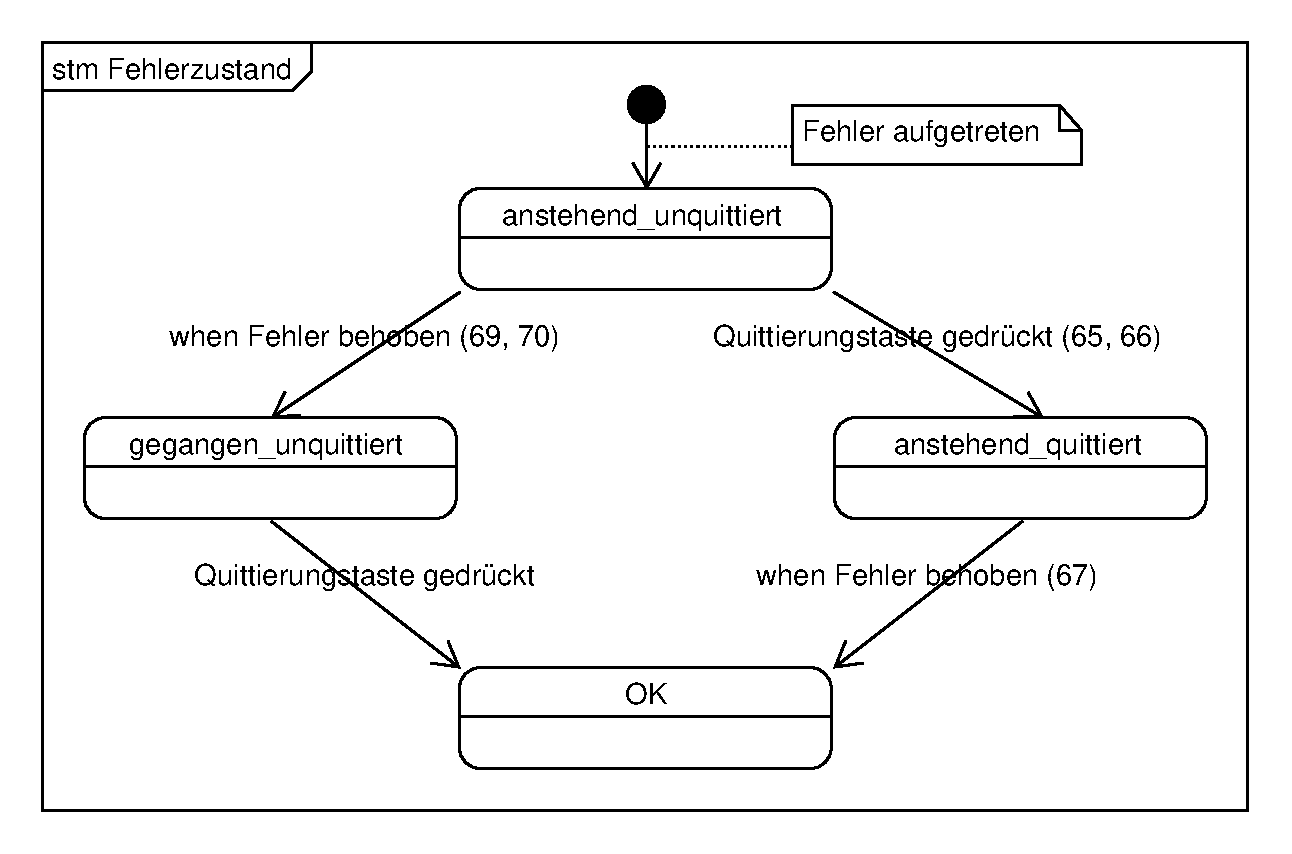
\includegraphics[scale=0.5]{../out/diagrams/stage1/req-fehlerzustand}
    \caption{REQ-36 Visualisierung des Fehlerzustandes eines einzelnen Fehlers}
    \label{fig:stm-fehlerzustand}
\end{figure}

\FloatBarrier

%% In der Aufgabenstellung sind Anforderungen an das System gestellt.
%% Arbeiten Sie diese hier auf und ergänzen Sie diese entsprechend der Absprachen mit dem Betreuer.
%% Achten Sie auf die entsprechende Atribuierung.
%% Berücksichtigen Sie auch mögliche Fehlbedienungen und Fehlverhalten des Systems.

\subsection{Systemkontext}\label{subsec:systemkontext2}

\begin{figure}
    \centering
    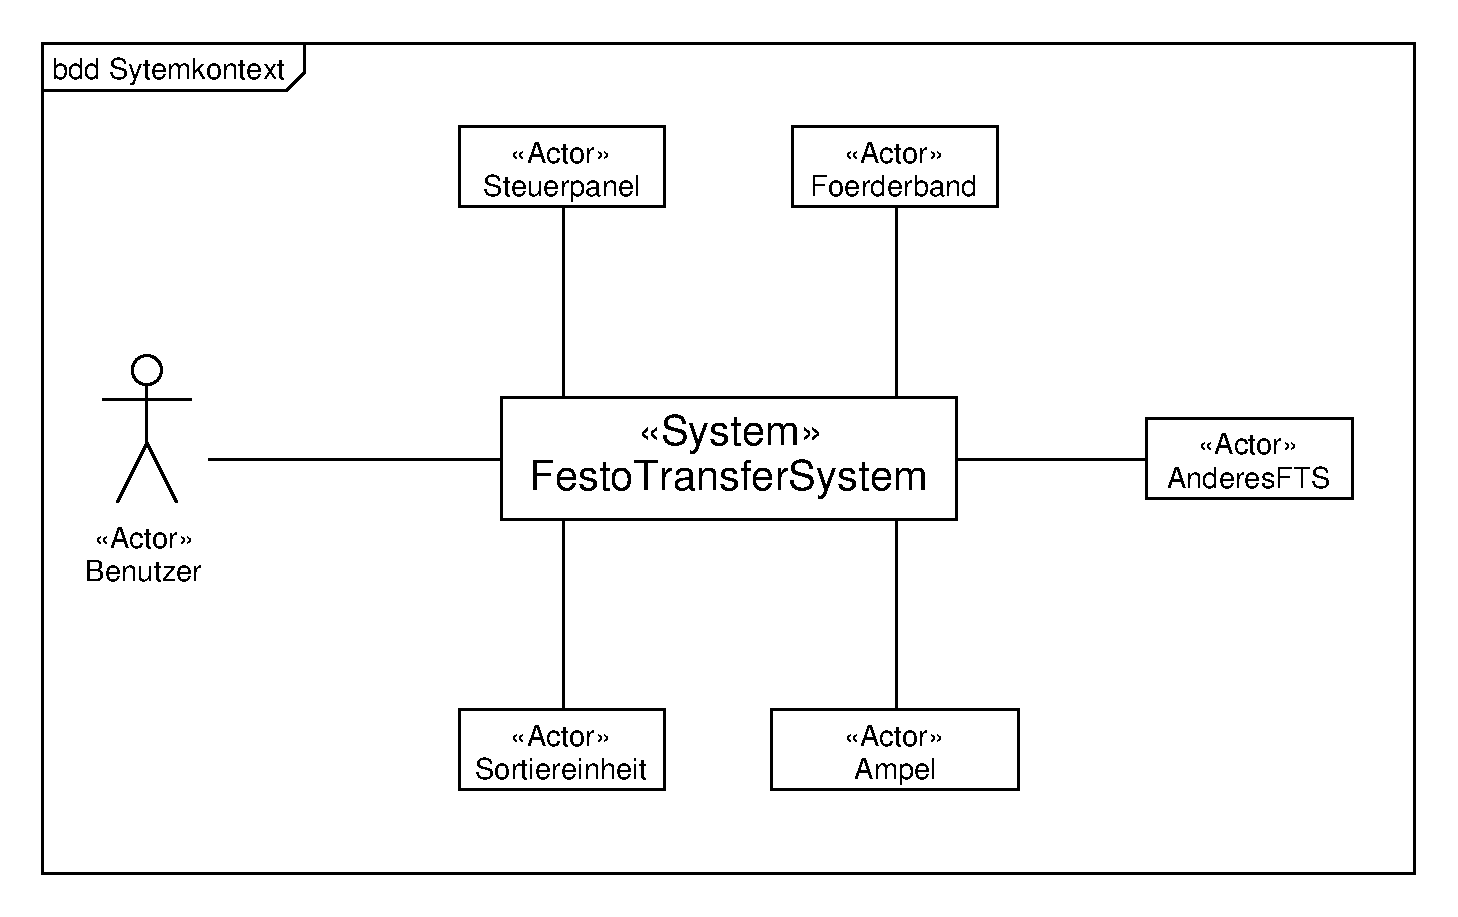
\includegraphics[width=\textwidth]{../out/diagrams/stage1/systemkontext.pdf}
    \caption{Systemkontext}
    \label{fig:systemkontext}
\end{figure}


Betrachte Abbildung \ref{fig:systemkontext}.
Die Systemsicht bringt umliegende Aktorik des Systems und System selber miteinander in Beziehung.

%% Use Cases werden aus einer bestimmten Sicht erstellt.
%% Dokumentieren Sie diese mittels Kontextdiagramm oder Use Case Diagramm.
%% Die Use Cases und Test Cases müssen zu der hier verwendeten Nomenklatur konsistent sein.

\subsection{Use Cases / User Stories}\label{subsec:use-cases-user-stories}

In Abbildung~\ref{fig:ucd} sind die Use Cases in einem Use Case Diagramm dargestellt.
Die Farbgebung dient lediglich zur Veranschaulichung.

\begin{figure}[h]
    \centering
    \makebox[\textwidth][c]{\includegraphics[width=1.2\textwidth]{../out/diagrams/stage1/ucd}}
    \caption{Use Case Diagramm}
    \label{fig:ucd}
\end{figure}

%% Dokumentieren Sie hier, welche Use Cases/ User Stories Sie auf der Systemebene implementieren müssen.
%% Die Test Cases sollen später zu den Use Cases/ User Stories konsistent sein.

%% < Hier kommt die genaue Beschreibung der Use.
%% Pro Anforderung eine Tabelle benutzen. Die Tabelle nach Belieben vervielfältigen. >


\begin{usecase}{02}{Determine Sorting Action}{hoch}
    \addCollum{Precondition}{
        \item Dem workpiece ist ein workpiece\_type zugeordnet
    }
    \addCollum{Actors}{
        \item LightBarrier\_Ramp
    }
    \addTextCollum{Description}{
        Es wird bestimmt, ob ein workpiece aussortiert werden soll, oder nicht.
        Dafür muss der Vorgänger workpiece\_type gespeichert werden.
    }
    \addCollum{Main flow}{
        \item[1)] Der aktuelle workpiece\_type wird mit dem erwarteten verglichen
        \item[2)] Das workpiece stimmt nicht überein, das workpiece muss aussortiert werden \textbullet
        \item[3)] Das workpiece wird mit discard markiert \textbullet
    }
    \addCollum{Alternative flow 1}{
        \item at step 2 of main flow
        \item[2a)] Das workpiece stimmt überein
        \begin{itemize}
            \item[2a1)] Das workpiece wird mit do\_not\_discard markiert
            \item[2a2)] Ende des use case
        \end{itemize}
    }
    \addCollum{Alternative flow 2}{
        \item at step 3 of main flow
        \item[3a)] Rutsche ist voll und in Primary mode
        \begin{itemize}
            \item[3a1)] das Teil mit do\_not\_discard markiert
        \end{itemize}
        \item[3b)] Rutsche ist voll und in Secondary mode
        \begin{itemize}
            \item[3b1)] Gesamtbetrieb wird gestoppt (REQ-6)
        \end{itemize}
    }    
    \addTextCollum{Postcondition}{
        Dem workpiece ist entweder do\_not\_discard oder discard zugeordnet
    }
    \addTextCollum{Verwandte Requirements}{
        REQ-1, REQ-2, REQ-3, REQ-6
    }
\end{usecase}


\begin{usecase}{03}{Handle Lightbarrier\_Switch}{hoch}
    \addTextCollum{Description}{
        Bindeglied zwischen \nameref{uc:02}, \nameref{uc:06} und \nameref{uc:15},
    }
    \addTextCollum{Trigger}{
        Light\_Barrier\_Switch unterbrochen
    }
    \addCollum{Mainflow}{
        \item[1)] UC2 determine sorting action
        \item[2)] Sorting action ist \gls{discard} \textbullet
        \item[3)] UC6 \gls{discard}
    }
    \addCollum{Alternate flow}{
        \item at step 2) of Mainflow
        \item[2a)] Sorting action ist \gls{do_not_discard}\_workpiece
        \begin{itemize}
            \item[2a1)] UC15 \gls{do_not_discard}\_workpiece
            \item[2a1)] Ende des use cases
        \end{itemize}
    }
    % postconditions sind in den jeweiligen unter UCs gehandelt.
\end{usecase}


\begin{usecase}{04}{Transfer Workpiece}{mittel}
    \addTextCollum{Verwandte Requirements}{
    REQ-9, REQ-14, REQ-16, REQ-18, REQ-31
    }
    \addTextCollum{Description}{
    In diesem Use-Case erreicht ein Werkstück das Ende eines Förderbandes und wird gegebenenfalls an das nächste Förderband transferiert
    }
    \addTextCollum{Actors}{
    Conveyor\_Belt, FTS\_2, LightBarrier\_End
    }

    \addCollum{Precondition}{
    \item Anlage befindet sich im Betriebszustand
    }

    \addCollum{Trigger}{
    \item LightBarrier\_End wird unterbrochen
    }

    \addCollum{Mainflow}{
    \item[1)] Die Anlage ist in Primary Mode \textbullet
    \item[2)] Conveyor\_Belt stoppen
    \item[3)] Anfrage zum transferieren und Werkstück\-Informationen an FTS\_2 senden
    \item[4)] Auf 'OK' von FTS\_2 warten
    \item[5)] Conveyor\_Belt in Bewegung setzen und Werkstück transferieren
    }

    \addCollum{Alternative Flow 1}{
    \item at step 1) of Mainflow
    \item[1a)] Die Anlage ist in Secondary Mode
    \begin{itemize}
        \item[1a1)] Ausgabe der ID, des Typs, Höhe\_FB1 und Höhe\_FB2 auf der Konsole
        \item[1a2)] Ausgabe an der Konsole, ob sich das Werkstück bei der Übergabe zwischen den Anlagen überschlagen hat
    \end{itemize}
    }

    \addCollum{Postcondition}{
    \item Werkstück ist nicht mehr auf dem Förderband
    }
\end{usecase}

%! Author = justi
%! Date = 23.04.2021

% Preamble
\documentclass[11pt]{article}

% Packages
\usepackage{amsmath}

% Document
\begin{document}



\end{document}

\begin{usecase}{06}{Discard workpiece}{hoch}
    \addTextCollum{Verwandte Requirements}{
        REQ-3, REQ-5, REQ-23, REQ-30, REQ-38, REQ-39
    }
    \addTextCollum{Description}{
    In diesem Use-Case bewegt der Aussortiertmechanismus der Anlage ein Werkstück vom Förderband in die Rutsche
    }
    \addTextCollum{Actors}{
    LightBarrier\_Switch, LightBarrier\_Ramp, SortingMechanism
    }
    \addCollum{Precondition}{
    \item Anlage befindet sich im Betriebszustand
    \item Dass das betroffene Werkstück aussortiert werden soll ist festgelegt
    }
    \addCollum{Trigger}{
    \item LightBarrier\_Switch unterbrochen
    }
    \addCollum{Mainflow}{
    \item[1)] Führe Aussortierung durch
    \item[2)] Warte auf Unterbrechung von LightBarrier\_Ramp
    \item[3)] LightBarrier\_Ramp wurde ausgelöst
    }

    \addCollum{Postcondition}{
    \item Werkstück liegt in der Rampe
    \item LightBarrier\_Switch nicht mehr unterbrochen
    }


    \addCollum{Exceptional flow 1}{
        \item at step 3) of Mainflow
        \item[1)] LightBarrier\_Ramp ist nach der 1,5-fachen durchschnittlichen Aussortierzeit nicht ausgelöst worden
        \item[2)] Warnung wird gesendet
    }
    \addCollum{Postcondition of e.f.}{
        \item LightBarrier\_Switch nicht mehr unterbrochen
        \item Eine Warnung über das Feststecken des Werkstückes liegt vor
    }
\end{usecase}

\begin{usecase}{07}{E-Stop}{hoch}
    \addCollum{Verwandte Requirements}{
    \item REQ-41, REQ-42, REQ-28,
    }
    \addTextCollum{Description}{
        Dieser Use-Case beschreibt den Umgang des Systems bei Betätigung des E-Stop-Schalters.
    }
    \addCollum{Actors}{
    \item E\_Stop, FTS\_2, Stoplight, Control\_Panel, Sorting\_Mechanism, Conveyor\_Belt
    }
    \addCollum{Precondition}{}
    \addCollum{Triggers}{
        \item[1a)] E\_Stop-Taster von FTS wird betätigt
        \item[1b)] E\_Stop-Schalter von FTS\_2 wird betätigt
    }
    \addCollum{Mainflow}{
        \item[1)] Der aktuelle Zustand sämtlicher Sensoren und Aktoren von FTS und FTS\_2 wird gespeichert
        \item[2)] Conveyor\_Belt, Sorting\_Mechanism von FTS und FTS\_2 werden abgeschaltet.
        \item[3)] Die Lampe am FTS und FTS\_2 leuchtet dauerhaft rot.
        \item[4)] E\_Stop-Schalter von FTS wird herausgezogen
        \item[5)] Reset-Taster von FTS wird gedrückt
    }
    \addCollum{Alternate flow}{
        \item at step 4) of Mainflow
        \item[2a)] E\_Stop-Schalter von FTS\_2 wurde betätigt
        \begin{itemize}
            \item[2a)] E\_Stop-Schalter von FTS\_2 wird herausgezogen
            \item[2b)] Reset-Taster von FTS\_2 wird gedrückt
        \end{itemize}
    }
    \addCollum{Postcondition}{
    \item Das System befindet sich im Ruhezustand.
    }
\end{usecase}

\begin{usecase}{08}{Switch To Idle}{mittel}
    \addTextCollum{Verwandte Requirements}{
        REQ-17, REQ-40
    }
    \addTextCollum{Description}{
        Dieser Use-Case beschreibt, wie vom Betriebszustand in den Ruhezustand, bzw. idle
        gewechselt wird.
    }
    \addCollum{Actors}{
        \item Sorting\_Mechanism
        \item Stoplight
        \item Control\_Panel
        \item FTS\_2
        \item Conveyor\_Belt
    }
    \addCollum{Precondition}{
        \item Es sind keine Fehler oder Warnungen vorhanden
        \item System ist im Betriebszustand
    }
    \addCollum{Triggers}{
        \item[1a)] Stopp-Taster am Control\_Panel betätigt
        \item[1b)] Event Request\_Idle von FTS\_2
    }
    \addCollum{Mainflow}{
        \item[1)] Zustand sämtlicher Sensoren und Aktoren wird gespeichert \textbullet
        \item[2)] Lampen an FTS und FTS\_2 wechseln auf gelb leuchtend
        \item[3)] LED am Start-Taster vom Control\_Panel ausschalten
        \item[4)] LED am Stopp-Taster vom Control\_Panel einschalten \textbullet
    }
    \addCollum{Alternative FLow 1}{
        \item at step 1 of Mainflow
        \item[1a)] Trigger war 1a)
        \begin{itemize}
            \item[2a1)] Request\_Idle wird an FTS\_2 gesendet
            \item[2a2)] Auf Ackknowledge von FTS\_2 warten \textbullet
            \item[2a3)] mit step 1 of Mainflow weitermachen
        \end{itemize}
    }
    \addCollum{Alternative Flow 2}{
        \item at step 4 of Mainflow
        \item[4a)] Trigger war 1b)
        \begin{itemize}
            \item[4a1)] Ackknowledge wird an FTS\_2 gesendet
        \end{itemize}
    }
    \addCollum{Exceptional Flow 1}{
        \item at Step 2a2 of Alternative Flow 1
        \item[2a)] Timeout beim Warten auf Ackknowledge
        \begin{itemize}
            \item[2a1)] Fehler auslösen
        \end{itemize}
    }
    \addCollum{Postcondition for Exceptional Flow 1}{
        \item System ist im Fehlerzustand
    }
    \addCollum{Postcondition}{
        \item System ist im Ruhezustand
    }
\end{usecase}

\begin{usecase}{09}{Start System}{hoch}
    \addTextCollum{Verwandte Requirements}{
        REQ-12, REQ-42
    }
    \addTextCollum{Actors}{
        FTS\_2, Control\_Panel
    }
    \addCollum{Preconditions}{
        \item System ist gestoppt
        \item System ist nicht im Fehlerzustand
    }
    \addCollum{Trigger}{
        \item Der Startknopf auf dem Steuerpanel wird gedrückt
        \item FTS\_2 schickt signal zum Starten
    }
    \addCollum{Mainflow}{
        \item[1)] System wechselt in den Betriebszustand \textbullet
        \item[2)] LED im Stopptaster wird ausgeschaltet
        \item[3)] LED im Starttaster wird eingeschaltet \textbullet
    }
    \addCollum{Alternate flow 1}{
        \item at step 1 of Mainflow
        \item[1)] Trigger ist Drücken des Knopfes
        \item[2)] Signal zum Starten an FTS\_2 schicken
        \item[3)] Auf Bestätigung von FTS\_2 warten \textbullet
        \item[4)] mit Mainflow Step 1 weitermachen
    }
    \addCollum{Alternate flow 2}{
        \item at step 3 of Mainflow
        \item[1)] Trigger ist Signal von FTS\_2 des Knopfes
        \item[2)] Signal Bestätigung an FTS\_2 schicken
    }
    \addCollum{Postconditions}{
        \item[2)] FTS\_2 ist im Betriebszustand
        \item[3)] System ist im Betriebszustand
    }
    \addCollum{Exceptional flow 1}{
        \item at step 3 of Alternate Flow 1
        \item[1)] Timeout
        \item[2)] In Fehlerzustand wechseln
    }
\end{usecase}


\begin{usecase}{10}{UseCase Bootup Configuration}{hoch}
    \addCollum{Actors}{
        \item[] FTS_2
        \item[] Control_Panel
    }
    \addCollum{Preconditions}{
        \item[] System ist mit Strom versorgt und Hochgefahren
    }
    \addCollum{Mainflow}{
        \item[1)] HAL wird initialisiert
        \item[2)] Herstellen einer Verbindung zu FTS_2
        \item[3)] Kontrolleuchte 1 auf Control_Panel Blink_Slow aktivieren
        \item[4)] Warten auf Drücken des Startknopfes auf dem ControlPanel
        \item[5)] EVNT_SW_COMM_PRI_REQ an FTS_2 schicken
        \item[6)] Warten auf EVNT_SW_COMM_SEC_AKC von FTS_2
        \item[7)] Eigenen Betriebsmodus auf PRIMARY setzen
        \item[8)] EVNT_SW_COMM_PRI_AKC an FTS_2 schicken
        \item[9)] Kontrolleuchte 1 auf Control_Panel dauerhaft aktivieren
    }
    \addCollum{Alternate flow 1}{
        \item[] at step 4 of Mainflow
        \item[1)] Event EVNT_SW_COMM_PRI_REQ von FTS_2 Empfangen
        \item[2)] Eigenen Betriebsmodus auf SECONDARY setzen
        \item[3)] EVNT_SW_COMM_SEC_AKC an FTS_2 senden
        \item[4)] auf EVNT_SW_COMM_PRI_AKC von FTS_2 warten
        \item[5)] Eigenen Betriebsmodus auf SECONDARY setzen
        \item[6)] Kontrolleuchte 1 auf Control_Panel dauerhaft aktivieren 
    }
    \addCollum{Alternate flow 2}{
        \item[] at step 2 of Mainflow
        \item[1)] Verbindung schlägt fehl
        \item[3)] Zurück in Schritt 2 Mainflow 
    }
    \addCollum{Postconditions}{
        \item[1)] HAL ist initialisiert
        \item[2)] Verbindung mit FTS_2 hergestellt
        \item[3)] Betriebsmodus der Anlage ist festgelegt
    }
    \addCollum{Exceptional flow 1}{
        \item[] at step 1 of Mainflow
        \item[1)] Initialisierung der HAL schlägt fehl
        \item[2)] Fehlermeldung ausgeben
        \item[3)] System abschalten
    }
    \addCollum{Exceptional flow 2}{
        \item[] at step 6 of Mainflow
        \item[1)] Timeout beim Empfangen von EVNT_SW_COMM_SEC_AKC
        \item[2)] Fehler COMM_ERROR auslösen
    }
    \addCollum{Exceptional flow 3}{
        \item[] at step 4 of Alternate flow
        \item[1)] Timeout beim Empfangen von auf EVNT_SW_COMM_PRI_AKC
        \item[2)] Fehler COMM_ERROR auslösen
    }
\addTextCollum{Description}{
    Dieser Use Case beschreibt die Initialisierung des Systems, sowie die Bestimmung von Primary und Secondary-Anlage.
    Das Primary System wird bestimmt
    Verwendete Signale sind EVNT_SW_COMM_PRI_REQ (Sendendes System will Primary sein), 
    EVNT_SW_COMM_SEC_AKC (Acknoledgement vom Secondary nach Empfang) und EVNT_SW_COMM_PRI_AKC (Abschließender Handshake)
}
\end{usecase}

\begin{usecase}{11}{Run Service}{hoch}
    \addTextCollum{Verwandte Requirements}{
        REQ-11, REQ-15, REQ-40
    }
    \addTextCollum{Description}{
        Dieser Usecase betreibt das Durchführen des Servicemode. 
        Dieser kann durch das lange drücken des Starttasters von beiden Anlagen aus aktiviert werden.
        Im Servicemode werden die Höhenmesser kalibriert sowie die korrekte Funktion des Aussortiermechanismus geprüft
    }
    \addCollum{Actors}{
        \item Stoplight
        \item Height\_Measurement
        \item Control\_Panel
        \item Sorting\_Mechanism
    }
    \addCollum{Preconditions}{
        \item System ist im Ruhezustand
    }
    \addCollum{Triggers}{
        \item Start-taster wird lange gedrückt
        \item Mitteilung von FTS\_2 über Betreten des Service
    }
    \addCollum{Mainflow}{
        \item[1)] Mitteilung an FTS\_2 über Betreten des Service senden
        \item[2)] Stoplight grün blinken lassen
        \item[3)] Messung bei Height\_Measurement anfragen
        \item[4)] Auf Rückmeldung warten
        \item[5)] Bestimmten Wert als Nullwert im Height\_Measurement eintragen
        \item[6)] Sorting Mechanism aktivieren
        \item[7)] Auf Zustandsänderungssignal des Sorting\_Mechanism warten \textbullet
        \item[8)] Sorting Mechanism deaktivieren
        \item[9)] Auf Zustandsänderungssignal des Sorting\_Mechanism warten \textbullet
        \item[10)] In Betriebszustand wechseln
    }
    \addCollum{Postconditions}{
        \item[1)] System ist im Ruhezustand
        \item[2)] Height\_Measurement wurde kalibriert
    }
    \addCollum{Exceptional flow 1}{
        \item at step 6 or 8 of Mainflow
        \item[1)] Timeout beim Empfang des Signals
        \item[2)] Fehler auslösen
    }
    \addCollum{Postconditions of Exceptional Flow 1}{
        \item[1)] System ist im Fehlerzustand
    }
\end{usecase}


\begin{usecase}{12}{Handle Error}{hoch}
    \addTextCollum{Verwandte Requirements}{
        REQ-21, REQ-36, REQ-37, REQ-43, REQ-46
    }
    \addTextCollum{Actors}{
        Stoplight, Control\_Panel
    }
    \addTextCollum{Description}{
        Der ErrorHandler verwaltet alle Fehler, die im System auftreten. Immer wenn ein Fehler-Event ausgelöst wird,
        legt der ErrorHandler diese in eine Fehlerliste ab. Jeder Fehler hat einen Fehlerzustand,
        welcher wie in der Statemachine~\ref{fig:stm_fehler} beschrieben ist.
        Wenn der Reset-Taster gedrückt wird, werden alle Fehler in der Fehlerliste quittiert.
        Fehler gelten als behoben, wenn ein Event die Behebung des Fehlers meldet.
        Der Fehlerzustand der gesamten Anlage, somit auch die Anzeige der roten LED,
        wird durch den dem Fehler mit der höchsten Priorität in der Fehlerliste festgelegt. Die Fehlerzustände sind wie in Fehlerpriorität priorisiert.
        Ist der globale Fehlerzustand anstehend\_unquittiert oder anstehend\_quittiert,
        dann bleiben die Laufbänder beider Anlagen stehen und der Strom an den Aussortiermechanismen wird abgestellt.
    }
    \addCollum{Fehlerpriorität}{
        \item[1)] anstehend\_unquittiert. Wird durch ein dauerhaftes leuchten der roten LED signalisiert.
        \item[2)] anstehend\_quittiert. Wird durch wird durch schnelles Blinken (1 Hz) der roten LED signalisiert.
        \item[3)] gegangen\_quittiert . Wird durch wird durch langsames Blinken (0,5 Hz) der roten LED signalisiert.
    }
\end{usecase}

\begin{usecase}{14}{Measure Height}{hoch}
    \addTextCollum{Description}{
        Die Höhe eines workpieces wird gemessen und das Höhenprofil dessen bestimmt.
    }
    \addTextCollum{Actors}{
        Height\_Measurement
    }
    \addTextCollum{Trigger}{
        LightBarrier\_Height
    }
    \addCollum{Mainflow}{
        \item[1)] Messung bei Height\_Measurement anfragen
        \item[2)] Auf Rückmeldung warten
        \item[3)] Rückgabewert mit den in Höhenprofile erwähnten Werten vergleichen
        \item[4)] Rückgabewert fällt in einen der Bereiche (plus Toleranz) \textbullet
        \item[4)] Jeweiliges Höhenprofile zurückgeben
    }
    \addCollum{Exceptional Flow}{
        \item at item 4) of main flow
        \item[4)] Rückgabewert liegt außerhalb aller Bereiche
        \begin{itemize}
            \item Fehlermeldung ausgeben
        \end{itemize}
    }
    \addCollum{Additional Information}{
        \item Höhenprofile
        \begin{itemize}
            \item BOHRUNG 15,8 bis 16,4mm
            \item FLACH 21,0mm
            \item HOCH 25,0 bis 25,4mm
        \end{itemize}
    }
\end{usecase}


\begin{usecase}{15}{Do not discard}{hoch}
    \addTextCollum{Verwandte Requirements}{
        REQ-2, REQ-27
    }
    \addTextCollum{Description}{
        In diesem Use-Case wird ein Werkstück vom Aussortiermechanismus durchgelassen
    }
    \addTextCollum{Actors}{
        Sorting\_Mechanism, LightBarrier\_Switch
    }
    \addCollum{Precondition}{
        \item Die Anlage befindet sich im Betriebszustand
        \item Das betroffene Werkstück ist als 'no discard' markiert
    }

    \addCollum{Mainflow}{
        \item[1)] Öffne Sorting\_Mechanism
        \item[2)] Setze Sorting\_Mechanism zurück, wenn LightBarrier\_Switch nicht mehr unterbrochen
    }

    \addCollum{Postcondition}{
        \item Sorting\_Mechanism zurückgesetzt
        \item Werkstück nicht aussortiert
    }
\end{usecase}

\begin{usecase}{16}{Answer Transfer Request}{mittel}
    \addTextCollum{Verwandte Requirements}{
    REQ-9, REQ-14, REQ-16, REQ-18, REQ-31
    }
    \addTextCollum{Description}{
    In diesem Use-Case wird eine Transfer Request, die von der Master-Anlage ausgeht, von der Slave-Anlage beantwortet
    }
    \addTextCollum{Actors}{
    Conveyor\_Belt, FTS\_2, LightBarrier\_Height, LightBarrier\_Start
    }
    \addCollum{Precondition}{
    \item Anlage ist im Betriebszustand
    \item Anlage befindet sich im Secondary Mode
    }
    \addCollum{Trigger}{
    \item Transfer Request mit Workpiece-Info von FTS\_2
    }
    \addCollum{Mainflow}{
    \item[1)] Kein Werkstück befindet sich zwischen LightBarrier\_Start und LightBarrier\_Height \textbullet
    \item[2)] Sende 'OK' an FTS\_2
    }

    \addCollum{Alternative Flow 1}{
    \item at stept 1) of Mainflow
    \item[1a)] Es befindet sich ein Werkstück zwischen LightBarrier\_Start und LightBarrier\_Height
    \begin{itemize}
        \item[1a1)] Warten auf Unterbrechung von LightBarrier\_Height
        \item[1a1)] Go back to step 2) of Mainflow
    \end{itemize}
    }

    \addCollum{Postcondition}{
    \item Transfer Request beantwortet
    }
\end{usecase}

\begin{usecase}{17}{Detect Material}{hoch}
    \addTextCollum{Verwandte Requirements}{
        REQ-1, REQ-2, REQ-3
    }
    \addTextCollum{Description}{
        In diesem Use-Case wird das Material eines Werkstückes erfasst.
        Grundsätzlich wird angenommen, dass ein Werkstück aus Kunststoff ist.
    }
    \addTextCollum{Actors}{
        Metal\_Detector
    }
    \addCollum{Precondition}{
        \item Die Anlage befindet sich im Betriebszustand
    }
    \addCollum{Trigger}{
        \item Metal\_Detector erfasst Metall
    }
    \addCollum{Mainflow}{
        \item[1)] Aktuellem Werkstück wird 'Metall' als Material zugewiesen
    }
    \addCollum{Postcondition}{
        \item Werkstück wurde Material 'Metall' zugewiesen
    }
\end{usecase}




\section{Systemanalyse}\label{sec:systemanalyse}

%% Ihr technisches System hat aus Sicht der Software bestimmte Eigenschaften.
%% Was muss man für die Entwicklung der Software in Struktur, Schnittstellen,
%% Verhalten und an Besonderheiten wissen?
%% Wählen Sie eine Kapitelstruktur, die am besten zur Dokumentation Ihrer Ergebnisse geeignet ist.

\subsection{Art des Systems}

Bei dem zu entwerfenden System handelt es sich um die Steuerung eines Festo-Transfersystems,
welche auf dem BeagleBoneBlack Einplatinencomputer, von dem jede Anlage einen besitzt, zu realisieren ist.
Daher handelt es sich um ein Embedded System.
Für das zu entwickelnde Softwaresystem bedeutet dies, dass es zur Steuerung der Prozesse sehr nah
an der in der Anlage verbauten Hardware arbeiten muss.
Ein weiterer wichtiger Punkt ist, dass das System mit einer weiteren gleichartigen Anlage über
das Netzwerk kommunizieren muss. Dies ist ebenfalls im Entwurfsprozess zu berücksichtigen.

\subsubsection{Eigenschaften des BeagleBoneBlack und Grundlagen QNX}

Auf dem BeagleBoneBlack Einplatinencomputer läuft das Echtzeitbetriebssystem QNX, das Kommunikation
zwischen Prozessen und Threads mittels Message Passing bevorzugt.
Dieses Message Passing kann auch über das Netzwerk erfolgen, sodass Messages auch an
einen weiteren BeagleBoneBlack geschickt werden können.
Die Architektur sollte sich daher auf Message-Passing stützen, gerade um die Kommunikation mit der
anderen gleichartigen Anlage zu erleichtern.
Da der BeagleBoneBlack ein eigenes Stück Hardware mit eigenem Betriebssystem ist, muss für die
Entwicklung die Entwicklungsumgebung QNX Momentics benutzt werden, die Debugging und Testing ermöglicht.
Die Kommunikation mit dem BeagleBoneBlack und dem Entwicklungsrechner erfolgt über die Netzwerkverbindung.

\subsection{Kommunikation mit der Hardware}

Die Ansteuerung der Aktorik und Sensorik der Anlage erfolgt direkt über die GPIOs des BeagleBoneBlack.
Die Sensorik ist hierbei an GPIO0, die Aktorik des Transfersystems an GPIO1 und die LEDs des Bedienpanels an GPIO2
gekoppelt.
Bei den GPIOs können Bits einzeln gesetzt und gelöscht werden und es können die aktuellen Werte ausgelesen werden.
Auf Veränderung an den GPIOs kann mittels pro Pin konfigurierbarer Interrupts (steigende Flanke, fallende Flanke,
Level=0, Level=1) reagiert werden.
Interrupts lassen sich nach dem Auslösen für einen einstellbare Zeit ignorieren (Debouncing).
Um später nicht direkt mit den GPIOs interagieren zu müssen, sollte ein Hardware Abstraction Layer
einfachere Schnittstellen zum Ansteuern der Aktorik und für das Reagieren auf die Sensorik bereitstellen.
Der Höhensensor ist am ADC des BeagleBoneBlack angeschlossen. Dieser kann über das Schreiben in ein
bestimmtes GPIO-Register aktiviert werden und kann dann nach erfolgreicher Messung einen Interrupt auslösen.

\subsection{Besonderheiten beim Systemaufbau}

Bei genauerer Betrachtung des Systemaufbaus fallen folgende Eigenschaften und Zusammenhänge besonders auf.
Sie sind bei der Verhaltensmodellierung zu berücksichtigen und könnten das Erkennen von Szenarien vereinfachen.

\subsubsection{Platzierung der Lichtschranke bei der Höhenmessung}

Die Lichtschranke an der Höhenmessung ist so platziert, dass sich die Mitte eines Werkstücks bei ihrer
Unterbrechung genau unter dem Höhenmesser befindet.
Auf diese Art lassen sich die unterschiedlichen Höhen von Werkstücken mittels einer einzelnen Messung unterscheiden.
Die gemessenen Höhen bei unterschiedlichen Werkstückarten gehen aus Tabelle~\ref{tab:werkstuecke} hervor.

\begin{table}[h]
    \begin{center}
        \begin{tabular}{ |c|c| }
            \hline
            Form                     & Höhe in mm \\
            \hline\hline
            HOCH                 &  25,0-25,4\\
            \hline
            FLACH                     & 19,8-20,2 \\
            \hline
            LOCH               & 15,8-16,4 \\
            \hline
        \end{tabular}
    \end{center}
    \caption{Höhen der unterschiedlichen Werkstückarten}
    \label{tab:werkstuecke}
\end{table}

Ebenso fällt auf, dass der Abstand der Lichtschranke für die Höhenmessung vom Anfang des Förderbands ca. 25 cm beträgt, 
was für die Bestimmung des Abstands bei der Werkstückübergabe zwischen zwei Anlagen wichtig ist.

\subsubsection{Der Aufbau im Bereich des Aussortiermechnaismus}

Im Transportweg der Werkstücke befindet sich an der Stelle, an der ein Werkstück vom Sortiermechanismus aussortiert
werden muss, eine Lichtschranke.
Das Unterbrechen dieser Lichtschranke kann daher als Signal zum Starten des Aussortiervorgangs verstanden werden.
Im Falle einer Weiche als Aussortiermechanismus müsste diese geöffnet werden, falls keine Aussortierung erfolgen soll.
Im Falle eines Auswerfers müsste dieser aktiviert werden, falls das Werkstück aussortiert werden muss.
Oberhalb des Werkstücks befindet sich in dieser Position auch der Metallsensor.
Bei einer Anlage mit Weiche ist wichtig, dass diese bei längerem Verharren im geöffneten Zustand beschädigt werden kann.

\section{Softwareebene}\label{sec:softwareebene}

%% Sie sollen Software für die Steuerung des technischen Systems erstellen.
%% Aus den Anforderungen auf der Systemebene und der Systemanalyse ergeben sich
%% Anforderungen für Ihre Software.
%% Insbesondere wird sich die Software der beiden Anlagenteile in einigen Punkten unterscheiden.
%% Dokumentieren Sie hier die Anforderungen, die sich speziell für die Software ergeben haben.

\subsection{Systemkontext}\label{subsec:systemkontext}

%% Wie sieht der Kontext Ihrer Software aus? Wie erfolgt die Kommunikation mit Nachbarsystemen?
%% Liste der ein- und ausgehenden Signale/Nachrichten.

\subsection{Anforderungen}\label{subsec:anforderungen}

%% Welche wesentlichen Anforderungen ergeben sich aus den Systemanforderungen für Ihre Software?
%% Berücksichtigen Sie auch mögliche Fehlbedienungen und Fehlverhalten des Systems.

    \clearpage
    \chapter{Design}\label{ch:design}

%% Anmerkung: Die Implementierung MUSS zu Ihrem Design-Modell konsistent sein.
%% Strukturen, Verhalten und Bezeichner im Code müssen mit dem Modell übereinstimmen.
%% Daher ist ein wohlüberlegtes Design wichtig.


\section{Systemarchitektur}\label{sec:systemarchitektur}

%% Erstellen Sie eine Architektur für Ihre Software.
%% Geben Sie eine kurze Beschreibung Ihrer Architektur mit den dazugehörenden Komponenten
%% und Schnittstellen an.
%% Dokumentieren Sie hier wichtige technische Entscheidungen.
%% Welche Pattern werden gegebenenfalls verwendet? Wie erfolgt die interne Kommunikation?

In Abbildung~\ref{fig:cmp} ist die Systemarchitektur mithilfe eines UML Komponentendiagramms
visualisiert.

\begin{figure}[h]
    \centering
    \makebox[\textwidth][c]{\includegraphics[width=1.2\textwidth]{../out/diagrams/stage1/cmp}}
    \caption{Komponentendiagramm}
    \label{fig:cmp}
\end{figure}

\begin{figure}
    \makebox[\textwidth][c]{\includegraphics[width=1.25\textwidth]{../out/diagrams/stage2/cd_hal}}
    \caption{Klassendiagramm HAL}
    \label{fig:cd-hal}
\end{figure}

\begin{figure}
    \makebox[\textwidth][c]{\includegraphics[width=1.25\textwidth]{../out/diagrams/stage3/cd_hal_sens}}
    \caption{}
    \label{fig:cd-hal-sens}
\end{figure}

\begin{figure}
    \makebox[\textwidth][c]{\includegraphics[width=1.25\textwidth]{../out/diagrams/stage3/cd_dispatcher}}
    \caption{Klassendiagramm Dispatcher}
    \label{fig:cd-dispatcher}
\end{figure}


\section{Datenmodellierung}\label{sec:datenmodellierung}

%% Bestimmen Sie das Datenmodell und dokumentieren Sie es hier mit Hilfe von UML Klassendiagrammen
%% unter Beachtung der Designprinzipien. Die Modelle können mit Hilfe eines UML-Tools erstellt werden.
%% Hier ist dann ein Übersichtsbild einzufügen.
%% Geben Sie eine kurze textuelle Beschreibung des Datenmodells
%% und deren wichtigsten Klassen und Methoden an.


\section{Verhaltensmodellierung}\label{sec:verhaltensmodellierung}

\subsection{Beschreibung des Servicemode}

Die detaillierte Durchführung des Servicemode ist in untenstehende Schritte unterteilt. Dabei ist mit der Quittierung
durch den Benutzer das Drücken des \gls{t_reset}s am \gls{ctrlp} gemeint.
\begin{enumerate}

    \item[1)] System schaltet \gls{ampelled} auf schnell grün blinkend
    \item[2)] Kalibrierung des \gls{lb_he}
    \begin{itemize}
        \item Der \gls{lb_he} wird kalibriert
        \item LED am \gls{t_reset} wird aktiviert
        \item Benutzer quittiert Kalibrierung der \gls{lb_he}
        \item LED am \gls{t_reset} wird deaktiviert
    \end{itemize}
    \item[3)] Testen des \gls{belt}s
    \begin{itemize}
        \item \Gls{belt} fährt für eine Sekunde schnell vorwärts
        \item \Gls{belt} fährt für eine Sekunde schnell rückwärts
        \item \Gls{belt} stoppt
        \item LED am \gls{t_reset} wird aktiviert
        \item Benutzer quittiert korrekte Funktionsweise des \gls{belt}s
        \item LED am \gls{t_reset} wird deaktiviert
    \end{itemize}
    \item[4)] Testen des \gls{sortierer}s
    \begin{enumerate}
        \item[4a)] \Gls{sortierer} ist \gls{weiche}
        \begin{itemize}
            \item \gls{weiche} wird für zwei Sekunden auf \gls{do_not_discard} gesetzt
            \item \gls{weiche} wird auf \gls{discard} gesetzt
            \item LED am \gls{t_reset} wird aktiviert
            \item Benutzer quittiert korrekte Funktionsweise der \gls{weiche}
            \item LED am \gls{t_reset} wird deaktiviert
        \end{itemize}
        \item[4b)] \gls{sortierer} ist \gls{ejector}
        \begin{itemize}
            \item \Gls{ejector} wird aktiviert
            \item LED am \gls{t_reset} wird aktiviert
            \item Benutzer quittiert korrekte Funktionsweise des \gls{ejector}s
            \item LED am \gls{t_reset} wird deaktiviert
        \end{itemize}
    \end{enumerate}
    \item[]

\end{enumerate}


\begin{figure}
    \makebox[\textwidth][c]{\includegraphics[height=0.93\textheight]{../out/diagrams/stage3/stm_top_level}}
    \caption{Der Einstiegspunkt einer \gls{anlage}.
    Verwaltet die Betriebszustände und Sub-State Machines}
    \label{fig:stm_top_level}
\end{figure}

\begin{figure}
    \makebox[\textwidth][c]{\includegraphics[width=1.25\textwidth]{../out/diagrams/stage3/stm_error}}
    \caption{Umgang mit Fehlern und Anzeige derer mithilfe der \gls{ampel}}
    \label{fig:stm_error}
\end{figure}

\begin{figure}
    \makebox[\textwidth][c]{\includegraphics[width=1.25\textwidth]{../out/diagrams/stage3/stm_werkstueck_annahme}}
    \caption{Die Annahme eines \glspl{workpiece}s am Anfang der \gls{anlage}}
    \label{fig:stm_werkstueck_annahme}
\end{figure}

\begin{figure}
    \makebox[\textwidth][c]{\includegraphics[width=1.25\textwidth]{../out/diagrams/stage3/stm_hoehe_messen}}
    \caption{Messung der Höhe eines \glspl{workpiece}s}
    \label{fig:stm_hoehe_messen}
\end{figure}

\begin{figure}
    \makebox[\textwidth][c]{\includegraphics[width=1.25\textwidth]{../out/diagrams/stage3/stm_werkstueck_sortieren}}
    \caption{Sortierung von \glspl{workpiece}n}
    \label{fig:stm_werkstueck_sortieren}
\end{figure}

\begin{figure}
    \makebox[\textwidth][c]{\includegraphics[width=1.25\textwidth]{../out/diagrams/stage3/stm_werkstueck_transfer}}
    \caption{Transfer eines \glspl{workpiece}s an die nächste \gls{anlage}}
    \label{fig:stm_werkstueck_transfer}
\end{figure}

\begin{figure}
    \centering
    \includegraphics[scale = 0.5]{../out/diagrams/stage3/stm_werkstueck_transfer_req_antworten}
    \caption{Antworten eines Transfer-Request der vorherigen \gls{anlage}.
    Ein Transfer-Request wird in stm Workpiece Transfer (Abbildung~\ref{fig:stm_werkstueck_transfer}) gesendet}
    \label{fig:stm_werkstueck_transfer_req_antworten}
\end{figure}


%% Ihre Software muss zur Bearbeitung der Aufgaben ein Verhalten aufweisen.
%% Überlegen Sie sich dieses Verhalten auf Basis der Anforderungen und modellieren
%% Sie das Verhalten unter Verwendung von Verhaltensdiagrammen aus den Vorlesungen.


    \clearpage
    \chapter{Implementierung}\label{ch:implementierung}

%% Anmerkung: Nur wichtige Implementierungsdetails sollen hier erklärt werden.
%% Code-Beispiele (snippets) können hier aufgelistet werden, um der Erklärung zu dienen.
%% Welche Patterns haben Sie für Ihre Implementierung benutzt.
%% Anmerkung: Bitte KEINE ganze Programme hierhin kopieren!


\section{Basis für STMs}\label{sec:basis-fuer-stms}

\begin{figure}[h]
    \centering
    \includegraphics[scale = 0.5]{../out/diagrams/stage3/cd_stm_base_classes}
    \caption{Basisklassen für die Implementierung der STMs}
    \label{fig:cd-stm-base}
\end{figure}

%TODO ^^^ text hierfür


\section{Embedded Recorder}\label{sec:embedded-recorder}

Die Record-Funktion des \gls{embRecer} nimmt alle Events der Sensorik auf und
speichert diese Events mit einem dazugehörigen Timestamp in einer json-Datei.
In den Programm-Argumenten kann mit \verb|--record=[filename]| bzw.
\verb|-R| die Record-Funktion aktiviert werden.
Die Events werden in eine json-Datei mit dem angegebenen Dateinamen geschrieben.
Wird kein Name angegeben, wird ein Timestamp als Dateiname verwendet.
Mit dem in C\# geschriebenen \gls{recCrea} können die erstellten
Eventaufzeichnungen eingelesen werden.
Das Programm erlaubt dem Benutzer die Aufzeichnungen zu bearbeiten.
Es gibt auch die Möglichkeit eine Eventabfolge neu zu erstellen.
\begin{figure}[h]
    \centering
    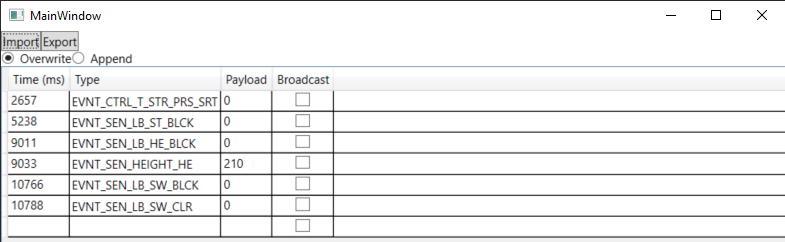
\includegraphics[scale = 0.7]{anhang/EmbeddedRecordCreator.PNG}
    \caption{Benutzeroberfläche des \gls{recCrea}}
    \label{fig:embedded-record-creator}
\end{figure}

\FloatBarrier
\noindent Die Replay-Funktion des \gls{embRecer} kann die Events einer json-Datei wieder
abspielen.
In den Programm-Argumenten wird mit \verb|-P [filename]| angegeben, dass eine bestimmte json-Datei
abgespielt werden soll.
Wenn die Replay-Funktion läuft, wird die Sensorik-HAL deaktiviert,
sodass die Sensoriksignale allein durch den \gls{embRecer} erstellt werden.
Diese Events werden an dem in der Datei gegebenen Timestamps zum Dispatcher gesendet.

    \clearpage
    \chapter{Testen}\label{ch:testen}

%% Machen Sie sich auf Basis Ihrer Überlegungen zur Qualitätssicherung Gedanken darüber,
%% wie Sie die Erfüllung der Anforderungen möglichst automatisiert im Rahmen von Teststufen
%% (Unit-Test, Komponententest, Integrationstest, Systemtest, Regressionstest und Abnahmetest)
%% überprüfen werden.


\section{Testplan}\label{sec:testplan}

%% Definieren Sie Zeitpunkte für die jeweiligen Teststufen in Ihrer Projektplanung.
%% Dazu können Sie die Meilensteine zu Hilfe nehmen.
%% Überlegen Sie, wie die Test-Architektur der jeweiligen Teststufen aussehen.
%% Verwenden Sie Testmethoden wie z.B.

%% Grenzwertanalyse
%% 100% Zustandsabdeckung
%% 100% Transitionsüberdeckung
%% Pfadüberdeckung
%% Tiefensuche
%% Breitensuche

%% Versuchen Sie, so gut wie möglich, Ihre Tests zu automatisieren.


\section{Testszenarien}\label{sec:testszenarien}

%% <konkrete Beschreibungen der Test Szenarien. Bei Bedarf die Tabelle vervielfältigen>
Für jede implementierte State-Machine wurden Unit-Tests geschrieben.
Diese Tests basieren auf den Abdeckungsbaum der jeweiligen State-Machine.
Mithilfe der Abdeckungsbäume wird sichergestellt, dass jeder Zustand getestet wird.
Dementsprechend wird auch ein möglichst großer Abdeckungsgrad sichergestellt.

\begin{figure}
    \makebox[\textwidth][c]{\includegraphics[width=1.25\textwidth]{../out/diagrams/stage3/tt_operation_manager}}
    \caption{Abdeckungsbaum der STM operation\_manager
        (Abbildung~\ref{fig:stm_operation_manager})}
    \label{fig:tt_operation_manager}
\end{figure}

\begin{figure}
    \makebox[\textwidth][c]{\includegraphics[width=1.25\textwidth]{../out/diagrams/stage3/tt_recieve_workpiece}}
    \caption{Abdeckungsbaum der STM receive\_workpiece
        (Abbildung~\ref{fig:stm_recieve_workpiece})}
    \label{fig:tt_recieve_workpiece}
\end{figure}

\begin{figure}
    \makebox[\textwidth][c]{\includegraphics[scale=0.5]{../out/diagrams/stage3/tt_height_measurement}}
    \caption{Abdeckungsbaum der STM height\_measurement
        (Abbildung~\ref{fig:stm_hoehe_messen})}
    \label{fig:tt_height_measurement}
\end{figure}

\begin{figure}
    \makebox[\textwidth][c]{\includegraphics[scale=0.5]{../out/diagrams/stage3/tt_sort_workpiece}}
    \caption{Abdeckungsbaum der STM sort\_workpiece
        (Abbildung~\ref{fig:stm_sort_workpiece})}
    \label{fig:tt_sort_workpiece}
\end{figure}

\begin{figure}
    \makebox[\textwidth][c]{\includegraphics[scale=0.5]{../out/diagrams/stage3/tt_workpiece_transfer}}
    \caption{Abdeckungsbaum der STM workpiece\_transfer
        (Abbildung~\ref{fig:stm_workpiece_transfer})}
    \label{fig:tt_workpiece_transfer}
\end{figure}

\begin{figure}
    \makebox[\textwidth][c]{\includegraphics[scale=0.5]{../out/diagrams/stage3/tt_workpiece_transfer_request}}
    \caption{Abdeckungsbaum der STM workpiece\_transfer\_request
        (Abbildung~\ref{fig:stm_workpiece_transfer_request})}
    \label{fig:tt_workpiece_transfer_request}
\end{figure}

\begin{figure}
    \makebox[\textwidth][c]{\includegraphics[scale=0.5]{../out/diagrams/stage3/tt_error_listener}}
    \caption{Abdeckungsbaum der STM error\_listener
        (Abbildung~\ref{fig:stm_error_listener})}
    \label{fig:tt_error_listener}
\end{figure}


\section{Abnahmetests}\label{sec:abnahmetest}

%% 6.3	Abnahmetest
%% Leiten Sie die Abnahmebedingungen aus den Kunden-Anforderungen her.
%% Dokumentieren Sie hier, welche Schritte für die Abnahme erforderlich sind
%% und welches Ergebnis jeweils erwartet wird (Test Cases).
%\begin{abntest}{Sortierung, Kapazität}{
    \refreq{1},
    \refreq{2},
    \refreq{3},
    \refreq{5},
    \refreq{13}, %<- TODO auslagern
    \refreq{30},
    \refreq{38},
    \refreq{39}
}{
    \item Das System befindet sich im Betriebszustand
    \item Falls nicht anders spezifiziert soll sichergestellt werden, dass
    \begin{enumerate}
        \item die \glspl{rampe}kapazität während der Tests nicht ausgeschöpft wird
        \item sich die \glspl{workpiece} während der Tests nicht überschlagen
    \end{enumerate}
}
    \label{abntest-sortierung-kapazitaet}

    \begin{ablauf}{Korrekte Reihenfolge}
        \item \Glspl{workpiece} in korrekter Reihenfolge einlegen:
        \begin{enumerate}[noitemsep, nolistsep]
            \item \gls{workpiece_metall}
            \item \gls{workpiece_bohrung}
            \item \gls{workpiece_flach}
            \item \gls{workpiece_metall}
        \end{enumerate}
    \end{ablauf}

    \erwartung
    Am Ende von \gls{anlage} 2 kommen die \Glspl{workpiece} in
    unveränderter Reihenfolge an (\refreq{2})

    \begin{ablauf}{Falsche Reihenfolge}
        \item Eine \gls{anlage} mit \gls{weiche}, die andere mit \gls{ejector} ausstatten
        (\refreq{30}, \refreq{38}, \refreq{39})
        \item \Glspl{workpiece} in falscher Reihenfolge einlegen:\label{enm:reih1}
        \begin{enumerate}[noitemsep, nolistsep]
            \item \gls{workpiece_hoch} %x
            \item \gls{workpiece_metall}
            \item \gls{workpiece_metall} %x
            \item \gls{workpiece_bohrung}
            \item \gls{workpiece_hoch} %x
            \item \gls{workpiece_flach}
            \item \gls{workpiece_bohrung} %x
            \item \gls{workpiece_metall}
        \end{enumerate}
        \item \Glspl{rampe}kapazität von \gls{anlage} 1 manuell ausschöpfen\label{enm:rampe1-voll}
        \item \Glspl{workpiece} in gleicher Reihenfolge wie in
        Schritt~\ref{enm:reih1} einlegen\label{enm:reih2}
        \item \Glspl{rampe}kapazität von \gls{anlage} 2 manuell ausschöpfen\label{enm:rampe2-voll}
    \end{ablauf}

    \erwartung
    \begin{enumerate}
        \item Bei Schritt~\ref{enm:reih1} und~\ref{enm:reih2}: Am Ende von \gls{anlage} 2 kommen
        \Glspl{workpiece} in folgender Reihenfolge an,
        alle anderen wurden aussortiert (\refreq{3})
        \begin{enumerate}[noitemsep, nolistsep]
            \item \gls{workpiece_metall}
            \item \gls{workpiece_bohrung}
            \item \gls{workpiece_flach}
            \item \gls{workpiece_metall}
        \end{enumerate}
        \item Nach Schritt~\ref{enm:rampe1-voll}  blinkt die gelbe \gls{ampelled}
        von \gls{anlage} 1 (\refreq{5}, \refreq{13})
        \item Nach Schritt~\ref{enm:rampe2-voll}  blinkt die gelbe \gls{ampelled}
        von \gls{anlage} 2 (\refreq{5}, \refreq{13})
    \end{enumerate}
    %todo: req 47 , 6
\end{abntest}

\abntest{Zustandsanzeigen}{
    \refreq{10},
    \refreq{11},
    \refreq{19},
    \refreq{45}
}{
    \item Das System befindet sich im Idle
}
\label{abntest-zustandsanzeigen}
\begin{anmerkungen}
    \item Die Anzeige von Fehlerzuständen wird in Abschnitt~\ref{abntest-fehlerumgang} getestet.
\end{anmerkungen}

\begin{ablauf}{Betriebszustände}
    \item \label{itm:to-service} Den Servicemodus betreten
    \item \label{itm:to-idle} Auf Rückkehr in den Idle warten
    \item \label{itm:to-betriebsz} Den Betriebszustand betreten
    \item \label{itm:to-idle2} Den Betriebszustand verlassen
\end{ablauf}
\begin{erwartung}
    \item Vor Schritt~\ref{itm:to-service} leuchten
    beide gelben \glspl{ampelled} dauerhaft, alle anderen sind aus (\refreq{45})
    \item Nach Schritt~\ref{itm:to-service} blinken
    beide grünen \glspl{ampelled}, alle anderen sind aus (\refreq{11})
    \item Nach Schritt~\ref{itm:to-idle} leuchten
    beide gelben \glspl{ampelled} dauerhaft, alle anderen sind aus (\refreq{45})
    \item Nach Schritt~\ref{itm:to-betriebsz} leuchten
    beide grünen \glspl{ampelled} dauerhaft, alle anderen sind aus (\refreq{10}, \refreq{19})
    \item Nach Schritt~\ref{itm:to-idle2} leuchten
    beide gelben \glspl{ampelled} dauerhaft, alle anderen sind aus (\refreq{45})
\end{erwartung}

\abntest{Fehlerumgang und Zustandsanzeigen}{
    \refreq{37},
    \refreq{43},
    \refreq{46} (indirekt durch \refreq{37}),
    \refreq{48}
}{
    \item Das System befindet sich im Idle
}
\label{abntest-fehlerumgang}

\begin{anmerkungen}
    \item Fehler erzeugen ist in diesem Abnahmetest wie folgt definiert:
    \begin{enumerate}
        \item In den Betriebszustand wechseln
        \item Kapazität beider \glspl{rampe} ausschöpfen
        \item Ein \gls{workpiece_hoch} einlegen
        \item Warten bis das \gls{workpiece_hoch} die \gls{lb_sw} erreicht
    \end{enumerate}
\end{anmerkungen}

\begin{ablauf}{Anstehened quittiert}
    \item \label{itm:1err} Fehler erzeugen
    \item\label{itm:1quitt} \gls{t_reset} drücken
    \item\label{itm:1ok} Die \gls{rampe} von \gls{anlage} 2 leeren
\end{ablauf}
\begin{erwartung}
    \item Nach Schritt~\ref{itm:1err}
    \begin{enumerate}
        \item bleiben die \glspl{belt} beider \glspl{anlage} stehen (\refreq{43})
        \item stehen beide \glspl{weiche} auf \gls{discard} (\refreq{48})
        \item blinkt die rote \gls{ampelled} schnell (\refreq{37}-\ref{req-37-unq})
    \end{enumerate}
    \item Nach Schritt~\ref{itm:1quitt} leuchtet die rote \gls{ampelled} dauerhaft (\refreq{37}-\ref{req-37-quit})
    \item Nach Schritt~\ref{itm:1ok} ist die rote \gls{ampelled} ausgeschaltet (\refreq{37}-\ref{req-37-ok})
\end{erwartung}

\begin{ablauf}{Gegangen unquittiert}
    \item \label{itm:2err} Fehler erzeugen
    \item\label{itm:2gegang} Die \gls{rampe} von \gls{anlage} 2 leeren
    \item\label{itm:2ok} \gls{t_reset} drücken
\end{ablauf}
\begin{erwartung}
    \item Nach Schritt~\ref{itm:2err}
    \begin{enumerate}
        \item bleiben die \glspl{belt} beider \glspl{anlage} stehen (\refreq{43})
        \item stehen beide \glspl{weiche} auf \gls{discard} (\refreq{48})
        \item blinkt die rote \gls{ampelled} schnell (\refreq{37}-\ref{req-37-unq})
    \end{enumerate}
    \item Nach Schritt~\ref{itm:2gegang} blinkt die rote \gls{ampelled} langsam (\refreq{37}-\ref{req-37-geg})
    \item Nach Schritt~\ref{itm:2ok} ist die rote \gls{ampelled} ausgeschaltet (\refreq{37}-\ref{req-37-ok})
\end{erwartung}

% TODO Fehler während quittiert oder unquittiert vorkommen lassen.

Die Abnahmetests liegen in einem
\href{https://docs.google.com/spreadsheets/d/1FzOZ4AyaUKZ6hcOzm9CIS6r-4n3aabzFG-6NZyX3wJg/edit?usp=sharing}{Google Sheets}
vor.


\section{Testprotokolle und Auswertungen}\label{sec:testprotokolle-und-auswertungen}

%% Hier fügen Sie die Test Protokolle bei, auch wenn Fehler bereits beseitigt worden sind,
%% ist es schön zu wissen, welche Fehler einst aufgetaucht sind.
%% Eventuelle Anmerkung zur Fehlerbehandlung kann für weitere Entwicklungen hilfreich sein.
%% Das letzte Testprotokoll ist das Abnahmeprotokoll, das bei der abschließenden Vorführung erstellt wird.
%% Es enthält eine Auflistung der erfolgreich vorgeführten Funktionen des Systems
%% sowie eine Mängelliste mit Erklärungen der Ursachen der Fehlfunktionen und  Vorschlägen zur Abhilfe

    \clearpage
    \chapter{Lessons Learned}\label{ch:lessons-learned}

%% Führen Sie ein Teammeeting durch, in dem gesammelt wird, was gut gelaufen war,
%% was schlecht gelaufen war und was man im nächsten Projekt (z.B. im PO) besser machen will.
%% Listen Sie für die Aspekte jeweils mindestens drei Punkte auf.
%% Weitere Erfahrungen und Erkenntnisse können hier ebenso kommentiert werden,
%% auch Anregungen für die Weiterentwicklung des Praktikums.
    \clearpage
    \appendix
    \chapter{Glossar}\label{ch:glossar}

%% Eindeutige Begriffserklärungen

%Glossary-Entries only show ub when referenced like this
%\gls{bsp1}
%\gls{bsp2}

\printnoidxglossary[type=abr]

\printnoidxglossary[type=term]

\printnoidxglossary[type=event]

\printnoidxglossary[type=var]
    \clearpage

\end{document}

